\chapter{Cross Plattform Frameworks}
Für die Realisierung eine Source-to-Source Compilers gibt es zwei relevante Faktoren,  die für die Realisierung ausschlaggebend sind.  Zum einen die Programmiersprachen in dem die beiden Frameworks entwickelt werden,  da bei der Übersetzung eine Brücke zwischen Quell und Zielsprache geschlagen werden muss.  Neben der Programmiersprache ist jedoch auch die Arbeitsweise eines Frameworks von essentieller Bedeutung.  Wie die Definition von Compilern bereits einführte,  müssen die Programme vor und nach der Übersetzung gleichwertig sein.  Dies implementiert,  dass das Verhalten der übersetzten Anwendungen nach der Übersetzung identisch seien muss wie das der Ursprungsanwendung.  Es ist also notwendig,  neben den sprachlichen auch die technischen Unterschiede zwischen den Frameworks zu kennen und diese im Rahmen der compilierung zu optimieren. 

\section{Frameworks}
Xamarin is eine Open Source-Plattform für das Erstellen mobiler Anwendungen für iOS und Android mit Hilfe des .NET Frameworks, welches von Microsoft weiterentwickelt wird.  Dabei ist Xamarin ist eine Abstraktionsebene, die die Kommunikation zwischen Code und dem zugrunde liegenden Plattformcode verwaltet.  Xamarin wird in einer verwalteten Umgebung ausgeführt, die Vorteile wie Speicherbelegung und Garbage Collection bietet.  Bei Xamarin.Forms handelt es sich um ein Open-Source-Benutzeroberflächenframework., mit dessen Hilfe Entwickler iOS- und Android- Anwendungen aus einer einzigen CodeBase erstellen können.  Dabei wird auf die in der .NET Welt bekannten Technologien XAML  für die Benutzeroberfläche und C\# für die Anwendungslogik zurückgegriffen.  Die einzelnen Benutzeroberflächen werden von Xamarin.Forms als native Steuerelemente auf jeder Plattform gerendert.  \footcite[Vgl.][Abgerufen am 28.10.2020]{MicrosoftWhatIsXam2020}

Flutter ist ebenfalls wie Xamarin.Forms ein Open Source Framework für die Erstellung von 2D mobilen Anwendungen.  Dabei werden im Vergleich zu Xamarin.Forms keine nativen Steuerelemente für jede Plattform gerendert sondern beinhaltet eine Sammlung von so genannten Widgets, die von dem Framework vewaltet und gerendert werden.  Für die Anzeige dieser Widgets wird auf die 2D engine Skia zugegriffen.  Flutter geht diesen Weg,  da das Endergebnis der Anwendungen eine höhere Qualität verspricht, da die nativen Steuerelemente in Bezug auf Flexibilität und Qualität begrenzt sind.  Außerdem ist es durch die Verwendung derselben Renderes einfacher, von derselben Codebasis aus für mehrere Plattformen zu veröffentlichen,  ohne eine sorgfältige und kostspielige Planung vornehmen zu müssen,  um verschiedene Funktionssätze und API-Merkmale aufeinander abzustimmen.\footcite[Vgl.][Abgerufen am 28.10.2020]{GoogleFlutterFAQ2020}

Dieser essentielle Unterschied zwischen den Frameworks werden in den folgenden Abschnitten dieser Arbeit deutlicher und sind bei der Übersetzung der Anwendungen fokussiert zu Berücksichtigen. 
\subsection{Projekte}
Xamarin.Forms Projektmappen setzen sich aus mehreren Projekten zusammen.  Zwei Projekten für jeweils iOS und Android,  welche den plattformspezifischen Code beinhalten sowie ein zusätzliches für den Quelltext,  der zwischen den Plattformen geteilt wird.  Im Gegensatz dazu gibt es bei Flutter nur ein Projekt, welches alle notwendigen Inhalte für iOS und Android beinhaltet.  Xamarin.Forms bietet Entwicklern die Möglichkeit über die plattformbezogenen Projekte die nativen Renderer zu manipulieren.  Durch diese sogenannten Custom Renderer (deutsch: benutzerdefinierter Renderer)ist es möglich unterschiedliche Darstellungen und Verhalten je nach Plattform zu erzeugen.  Flutter bietet diese Möglichkeit nicht, da wie bereits beschrieben ausschließlich einheitliche Renderer Angeboten werden. 

\subsection{Views}
Views (zu Deutsch Ansichten) sind visuelle Elemente die in zwei Kategorien unterschieden werden können.  Controls, die für die Sammlung von Benutzereingaben oder die Ausgabe von Daten sind.  Sowie Layouts die eine Sammlung von Ansichten beinhalten und für die Anordnung der untergeorderten Ansichten in der Benutzeroberfläche verantwortlich sind.  Außerdem arbeitet sie mit jeder untergeordneten Ansicht zusammen, um die endgültige Rendering-Größe zu bestimmen.\footcite[Vgl.][Abgerufen am 28.10.2020]{Ritscher2020}
\subsubsection{Pages}
Pages (zu Deutsch: Ansichtseiten) sind visuelle Elemente einer Anwendung die den gesamten Bildschirm belegen und zu den Layout Views gehören.  Xamarin Forms bietet dafür 
verschiedene Alternativen an,  die in \ref{fig:Xamarin.Forms Pages} grafisch dargestellt sind.\footcite[Vgl.][Abgerufen am 28.10.2020]{MicrosoftXamPages2016}

\begin{figure}[h]
 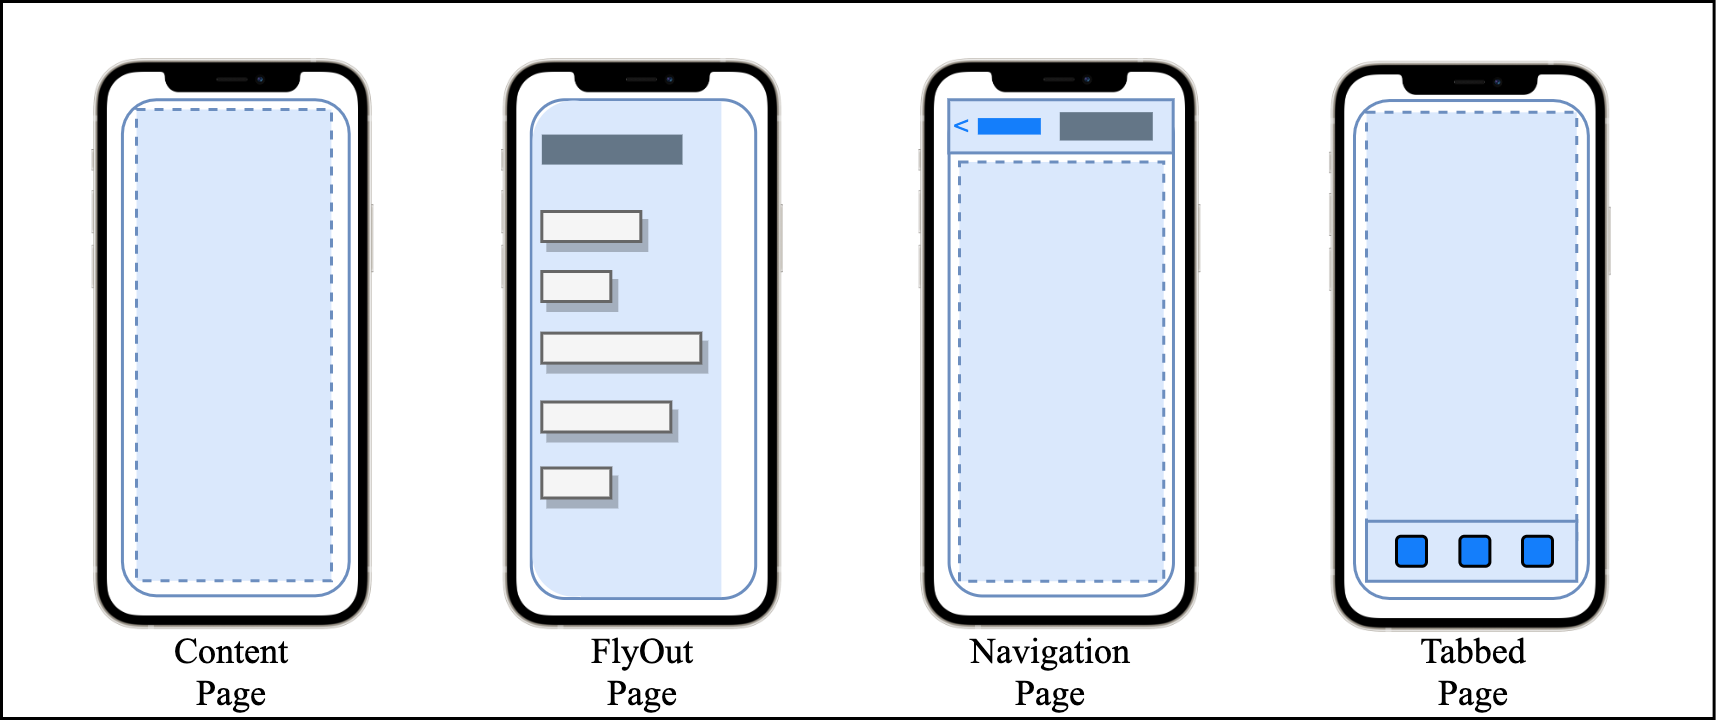
\includegraphics[width=\textwidth,height=\textheight,keepaspectratio]{Images/CrossPlattformFrameworks/XamarinFormsPages.png}
 \caption{Xamarin.Forms Pages}
 \label{fig:Xamarin.Forms Pages}
\end{figure}

Wie die Darstellung präsentiert, hat die Auswahl einer Page einen direkten Einfluss auf das Navigationskonzept innerhalb der Anwendung.  Abgesehen von der ContentPage, die ausschließlich eine View anzeigt haben die jeweiligen Seiten das folgende Navigationskonzept: 

\begin{itemize}
\setlength\itemsep{-0.6em}
 \item FlyOutPage: Eine Seite, die zwei Bereiche für die Seite hat. Typischerweise enthält das Flyout ein Menü über welches zwischen den eigentlichen Inhaltsseiten navigiert werden kann.
 \item NavigationPage: Eine Seite,  die eine Navigationsleiste enthält.  Die Seiten werden auf einem Stapel gehalten und es kann zwischen ihnen gesprungen werden.  Die Navigationsleiste kann sowohl Navigationsschaltflächen als auch einen Titel enthalten.
 \item TabbedPage: Eine Container-Seite.  Die TabbedPage fungiert als Container,  der die mit jeder Registerkarte verbundenen Inhaltsseiten enthält.
\end{itemize}

Die Auswahl einer Page wird innerhalb des Wurzelknoten der XAML Datei definiert.  Dies wird in Quelltext \ref{lst:TabbedPage} dargestellt. 

\begin{minipage}{\linewidth}
\lstinputlisting[label={lst:TabbedPage},caption={Xamarin.Forms TabbedPage definition}, language=XML]{SourceCode/XamarinFormsTabbedPage.XAML}
\end{minipage}

Das Beispiel zeigt eine TabbedPage mit drei in diesem Falle leeren NavigationsPages die als Children der TabbedPage hinzugefügt werden.  Im Gegensatz zu der TabbedPage hat die FlyoutPage keine Sammlung von ChildrenPages sondern ein sogenanntes "Flyout" welches das Menu beinhaltet und die entsprechend ausgewählte Seite in eine Detailansicht läd.  Dies wird in Quelltext \ref{lst:FlyOutPage} dargestellt.

\begin{minipage}{\linewidth}
\lstinputlisting[label={lst:FlyOutPage},caption={Xamarin.Forms FlyOut definition}, language=XML]{SourceCode/XamarinFormsFlyoutPage.XAML}
\end{minipage}

Im Gegensatz zu Xamarin.Forms lässt sich bei Flutter auf der Ebene der Wurzel kein Navigationskonzept definieren,  sondern ausschließlich das Style der Anwendung.  Flutter unterstützt drei alternativen: MaterialApp erzeugt eine App mit dem von Google entwickelten Material Design, CupertinoApp für eine App im iOS-Stil oder die Definition eines eigenen Styles für eine individuelle Anzeige.  \footcite[Vgl.][Abgerufen am 28.10.2020]{GoogleFlutterPages2020}  Quelltext \ref{lst:MaterialApp} zeigt die Definition einer MaterialDesign App in Flutter.

\begin{minipage}{\linewidth}
\lstinputlisting[label={lst:MaterialApp},caption={Flutter MaterialApp definition}, language=Dart]{SourceCode/MaterialApp.Dart}
\end{minipage}

Von diesem Widget aus ist die eigentliche erste Seite ein weiteres zustandsabhängiges Widget.  Dieses besteht aus zwei Teilen:  Der erste Teil, der selbst unveränderlich ist, erzeugt ein State-Objekt, das den Zustand des Objekts enthält.  Das State-Objekt bleibt während der Lebensdauer des Widgets bestehen.
Das State-Objekt implementiert die build()-Methode für das zustandsabhängige Widget.  Wenn sich der Zustand des Widget-Baums ändert,  wird setState() aufgerufen was einen Build des entsprechenden Teils der Benutzeroberfläche auslöst.  In Flutter ist die Benutzeroberfläche (auch bekannt als Widget-Baum) unveränderlich,  dass bedeutet da der Zustand nicht mehr geändert werden kann, sobald dieser aufgebaut ist.  Sie ändern Felder in Ihrer State-Klasse und rufen dann setState() auf, um den gesamten Widget-Baum neu zu erstellen. 

Damit die Navigation ähnlich wie in Xamarin.Forms definiert werden kann müssen verschiedene Widgets in einem Widget Baum verschachtelt werden.  Quelltext \ref{lst:FlutterTabbedApp} zeigt dies für die Arbeit mit Tabbs.  In diesem Beispiel wird eine TabBar mit drei Tab-Widgets erstellt und diese innerhalb einer AppBar platziert.\footcite[Vgl.][Abgerufen am 28.10.2020]{GoogleFlutterTabs2020} 

\begin{minipage}{\linewidth}
\lstinputlisting[label={lst:FlutterTabbedApp},caption={Flutter Tab Layout definition}, language=Dart]{SourceCode/TabbedPage.Dart}
\end{minipage}


\subsubsection{Layouts}

Layouts werden in Xamarin.Forms verwendet, um die Steuerelemente der Benutzeroberfläche zu visuellen Strukturen zusammenzustellen. Dabei unterscheidet man zwischen Layouts die ausschließlich einen oder mehrere Inhalte beinhalten können.  Xamarin.Forms bietet die folgende Layouts an:

\begin{itemize}
\setlength\itemsep{-0.6em}
 \item ContentView: ContentView enthält ein einzelnes untergeordnetes Element, das mit der Eigenschaft "Content" festgelegt wird. Die Eigenschaft Content kann auf jedes View-Derivat gesetzt werden, auch auf andere Layout-Derivate. ContentView wird meist als Strukturelement verwendet und dient als Basisklasse zu Frame.
 \item Frame: Die Klasse Frame leitet sich von ContentView ab und zeigt einen Rahmen um die Ansicht.
  \item ScrollView: Ist in der Lage, seinen Inhalt zu scrollen.  Die Eigenschaft Content auf eine Ansicht oder ein Layout fest, das zu groß ist, um auf den Bildschirm zu passen.  Legen Sie die Eigenschaft Orientierung fest, um anzugeben, ob der Bildlauf vertikal, horizontal oder beides sein soll.
 \item StackLayout: Positioniert untergeordnete Elemente in einem Stapel entweder horizontal oder vertikal, basierend auf der Eigenschaft Orientation.
 \item Grid: Grid positioniert seine untergeordneten Elemente in einem Raster aus Zeilen und Spalten. Die Position eines untergeordneten Elements wird über die angehängten Eigenschaften Row, Column, RowSpan und ColumnSpan angegeben.
 \item AbsolutLayout: Positioniert untergeordnete Elemente an bestimmten Positionen relativ zu ihrem übergeordneten Element. Die Position eines untergeordneten Elements wird über die angehängten Eigenschaften LayoutBounds und LayoutFlags angegeben. Ein AbsoluteLayout ist nützlich, um die Positionen von Ansichten zu animieren.
 \item RelativeLayout:  Positioniert untergeordnete Elemente relativ zum RelativeLayout selbst oder zu ihren Geschwistern. Die Position eines Kindelements wird über die angehängten Eigenschaften angegeben, die auf Objekte vom Typ Constraint und BoundsConstraint gesetzt werden.
\end{itemize}

Alle verfügbaren Layouts werden in  \ref{fig:Xamarin.Forms Layouts} grafisch dargestellt.

\begin{figure}[h]
 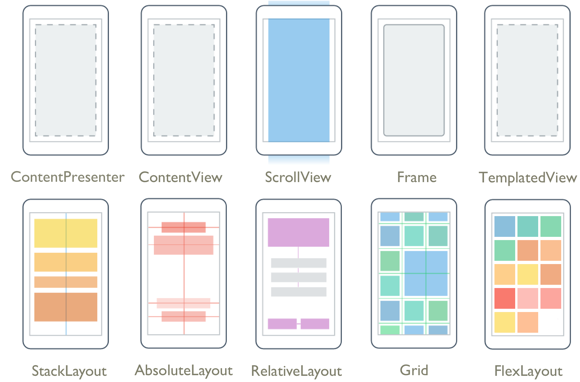
\includegraphics[width=\textwidth,height=\textheight,keepaspectratio]{Images/CrossPlattformFrameworks/XamarinFormsLayouts.png}
 \caption{Xamarin.Forms Layouts}
 \label{fig:Xamarin.Forms Layouts}
\end{figure}


\subsubsection{Steuerelemente}

Xamarin.Forms-Ansichten sind die Bausteine von plattformübergreifenden mobilen Benutzeroberflächen. Ansichten sind Objekte der Benutzeroberfläche wie Beschriftungen, Schaltflächen und Schieberegler, die in anderen grafischen Programmierumgebungen üblicherweise als Steuerelemente oder Widgets bezeichnet werden. Die von Xamarin.Forms unterstützten Ansichten leiten sich alle von der Klasse View ab. 
\subsubsection{Steuerelemente für die Darstellung}

\begin{itemize}
\setlength\itemsep{-0.6em}
 \item BoxView zeigt ein einfarbiges Rechteck an 
 \item Ellipse zeigt eine Ellipse oder einen Kreis an
  \item Label zeigt einzeilige Textstrings oder mehrzeilige Textblöcke an, entweder mit konstanter oder variabler Formatierung.
 \item Line zeigt eine Linie von einem Startpunkt zu einem Endpunkt an
 \item Image zeigt ein Bitmap an, diese können über das Web heruntergeladen, als Ressourcen in über das gemeinsame Projekt oder in Plattformprojekte eingebettet  werden
 \item Map zeigt eine Karte an
 \item OpenGLView zeigt OpenGL-Grafiken an
 \item Path zeigt Kurven und komplexe Formen an.
 \item Polygon Polygon zeigt ein Polygon an.
 \item  Polyline zeigt eine Reihe von verbundenen geraden Linien an
 \item Rectangle zeigt ein Rechteck oder Quadrat an
 \item WebView zeigt Web-Seiten oder HTML-Inhalte an
\end{itemize}

\subsubsection{Steuerelemente die Aktionen auslösen}

\begin{itemize}
\setlength\itemsep{-0.6em}
 \item Button ist ein rechteckiges Objekt, das Text anzeigt und ein Clicked-Ereignis auslöst, wenn es gedrückt wurde.
 \item ImageButton ist ein rechteckiges Objekt, das ein Bild anzeigt und ein Clicked-Ereignis auslöst, wenn es gedrückt wurde.
  \item RadioButton erlaubt die Auswahl einer Option aus einer Menge und feuert ein CheckedChanged-Ereignis, wenn die Auswahl erfolgt.
 \item RefreshView ist ein Container-Steuerelement, das eine Pull-to-Refresh-Funktionalität für scrollbare Inhalte bietet. 
 \item SearchBar zeigt einen Bereich an, in dem der Benutzer eine Textzeichenfolge eingeben kann, sowie eine Schaltfläche (oder eine Tastaturtaste), die der Anwendung signalisiert, eine Suche durchzuführen
 \item SwipeView ist ein Container-Steuerelement, das sich um ein Inhaltselement legt und Kontextmenüelemente bereitstellt, die durch eine Wischgeste angezeigt werden
\end{itemize}



\subsubsection{Steuerelemente um Werte zu setzen}


\begin{itemize}
\setlength\itemsep{-0.6em}
 \item CheckBox ermöglicht dem Benutzer die Auswahl eines booleschen Wertes mit Hilfe einer Art Schaltfläche, die entweder markiert oder leer sein kann
 \item Schieberegler bieten Benutzern die Option einen  Wert aus einem kontinuierlichen Bereich auswählen, der mit den Eigenschaften Minimum und Maximum festgelegt wurde.
 \item Stepper ermöglicht es dem Benutzer, einen doppelten Wert aus einem Bereich von inkrementellen Werten auszuwählen, die mit den Eigenschaften Minimum, Maximum und Inkrement festgelegt wurden.
 \item Schalter hat die Form eines Ein/Aus-Schalters, damit der Benutzer einen booleschen Wert auswählen kann
 \item DatePicker ermöglicht es dem Benutzer, ein Datum mit der Datumsauswahl der Plattform auszuwählen.
 \item TimePicker ermöglicht dem Benutzer die Auswahl einer Zeit mit dem TimePicker der Plattform
\end{itemize}
\subsubsection{Steuerelemente um text zu manipulieren}

\begin{itemize}
\setlength\itemsep{-0.6em}
 \item Entry ermöglicht dem Benutzer die Eingabe und Bearbeitung einer einzelnen Textzeile
 \item Editor ermöglicht dem Benutzer die Eingabe und Bearbeitung mehrerer Textzeilen
\end{itemize}
\subsubsection{Steuerelemente um eine Aktivität anzudeuten}


\begin{itemize}
\setlength\itemsep{-0.6em}
 \item ActivityIndicator verwendet eine Animation, um zu zeigen, dass die Anwendung eine langwierige Aktivität ausführt, ohne einen Hinweis auf den Fortschritt zu geben. 
 \item ProgressBar verwendet eine Animation, um zu zeigen, dass die Anwendung durch eine langwierige Aktivität fortschreitet
\end{itemize}

\subsubsection{Steuerelemente um Sammlungen anzuzeigen}
\begin{itemize}
\setlength\itemsep{-0.6em}
 \item CarouselView zeigt eine blätterbare Liste von Datenelementen an
 \item CollectionView zeigt eine scrollbare Liste mit auswählbaren Datenelementen an, wobei verschiedene Layout-Spezifikationen verwendet werden. Sie soll eine flexiblere und performantere Alternative zu ListView darstellen. 
  \item IndicatorView zeigt Indikatoren an, die die Anzahl der Elemente in einer CarouselView darstellen
 \item ListView zeigt eine scrollbare Liste mit auswählbaren Datenelementen an
 \item Picker zeigt ein ausgewähltes Element aus einer Liste von Textzeichenfolgen an und ermöglicht die Auswahl dieses Elements, wenn die Ansicht angetippt wird
 \item TableView zeigt eine Liste von Zeilen mit optionalen Überschriften und Unterüberschriften an
\end{itemize}

\subsubsection{Listen}
\subsubsection{Gesten}
\subsubsection{Animtion}

\subsection{Navigation}
In Xamarin.Forms bietet die Klasse NavigationPage eine hierarchische Navigation, bei der der Benutzer durch die Seiten, vorwärts und rückwärts, navigieren kann.

Flutter hat eine ähnliche Implementierung, die einen Navigator und Routen verwendet. Eine Route ist eine Abstraktion für eine Seite einer App, und ein Navigator ist ein Widget, das Routen verwaltet. Eine Route bildet grob eine Seite ab. Der Navigator arbeitet ähnlich wie die Xamarin.Forms NavigationPage, indem er Routen push() und pop() kann, je nachdem, ob man zu einer Ansicht hin oder von ihr zurück navigieren möchte.

\subsubsection{Navigation zu anderen Apps}
In Xamarin.Forms verwenden kann, um zu einer anderen Anwendung zu navigieren, ein bestimmtes URI-Schema verwendet werden.  So z.B. mit dem Befehl Device.OpenUrl("mailto://") das Standard E-Mail-Programm des Gerätes geöffnet werden verwenden.
Um diese Funktionalität in Flutter zu implementieren,  muss eine native Plattformintegration oder eine vorhandenes Plugin, wie z. B. urllauncher verwendet werden.  
\subsection{Async UI}
Dart hat ein Single-Thread-Ausführungsmodell mit Unterstützung für Isolates (eine Möglichkeit, Dart-Code in einem anderen Thread auszuführen), eine Ereignisschleife und asynchrone Programmierung. Sofern Sie kein Isolate erzeugen, wird Ihr Dart-Code im Haupt-Thread der Benutzeroberfläche ausgeführt und von einer Ereignisschleife gesteuert.

Das Single-Thread-Modell von Dart bedeutet nicht, dass Sie alles als blockierende Operation ausführen müssen, die das Einfrieren der Benutzeroberfläche verursacht. Ähnlich wie bei Xamarin.Forms müssen Sie den UI-Thread frei halten. Sie würden async/await verwenden, um Aufgaben auszuführen, bei denen Sie auf die Antwort warten müssen.

In Flutter verwenden Sie die asynchronen Möglichkeiten, die die Sprache Dart bietet, auch async await genannt, um asynchrone Arbeiten auszuführen. Dies ist C\# sehr ähnlich und sollte für jeden Xamarin.Forms-Entwickler sehr einfach zu verwenden sein.

Sie können zum Beispiel Netzwerkcode ausführen, ohne dass die Benutzeroberfläche hängen bleibt, indem Sie async await verwenden und Dart die schwere Arbeit erledigen lassen:
Sobald der erwartete Netzwerkaufruf erfolgt ist, aktualisieren Sie die Benutzeroberfläche durch den Aufruf von setState(), was einen Neuaufbau des Widget-Unterbaums auslöst und die Daten aktualisiert.
\subsection{Hintergrundarbeiten}
Da Flutter Single-Thread-fähig ist und eine Ereignisschleife ausführt, müssen Sie sich nicht um das Thread-Management oder das Erzeugen von Hintergrund-Threads kümmern. Dies ist sehr ähnlich wie bei Xamarin.Forms. Wenn Sie E A-gebundene Arbeiten durchführen, wie z. B. Festplattenzugriffe oder Netzwerkaufrufe, dann können Sie async await verwenden und alles ist bereit.

Wenn Sie andererseits rechenintensive Arbeiten ausführen müssen, die die CPU beschäftigen, sollten Sie sie in ein Isolate verschieben, um ein Blockieren der Ereignisschleife zu vermeiden, so wie Sie jede Art von Arbeit aus dem Hauptthread heraushalten würden. Dies ist ähnlich, wie wenn Sie Dinge über Task.Run() in Xamarin.Forms in einen anderen Thread verschieben.

Für E/A-gebundene Arbeit deklarieren Sie die Funktion als asynchrone Funktion und warten Sie auf lang laufende Aufgaben innerhalb der Funktion.

So würden Sie normalerweise Netzwerk- oder Datenbankaufrufe durchführen, die beide E/A-Operationen sind.

Es kann jedoch vorkommen, dass Sie eine große Datenmenge verarbeiten und Ihre Benutzeroberfläche hängen bleibt. In Flutter verwenden Sie Isolates, um die Vorteile mehrerer CPU-Kerne zu nutzen, um langlaufende oder rechenintensive Aufgaben zu erledigen.

Isolates sind separate Ausführungsthreads, die sich keinen Speicher mit dem Hauptspeicherheap der Ausführung teilen. Dies ist ein Unterschied zu Task.Run(). Das bedeutet, dass Sie vom Haupt-Thread aus nicht auf Variablen zugreifen oder Ihre Benutzeroberfläche durch den Aufruf von setState() aktualisieren können.
\subsection{Netzwerkaufrufe}
In Xamarin.Forms würden Sie HttpClient verwenden. Einen Netzwerkaufruf in Flutter zu machen ist einfach, wenn Sie das beliebte http-Paket verwenden. Dieses abstrahiert einen Großteil des Netzwerks, das Sie normalerweise selbst implementieren würden, und macht es einfach, Netzwerkaufrufe zu tätigen.

Um das http-Paket zu verwenden, fügen Sie es zu Ihren Abhängigkeiten in pubspec.yaml hinzu.

Um eine Netzwerkanfrage zu stellen, rufen Sie await auf die asynchrone Funktion http.get() auf:


\begin{minipage}{\linewidth}
\lstinputlisting[label={lst:FlutterFont},caption={Flutter Font definition}, language=Dart]{SourceCode/Fonts.Dart}
\end{minipage}

\subsection{Lebenzyklus}
In Xamarin.Forms haben Sie eine Anwendung, die OnStart, OnResume und OnSleep enthält. In Flutter können Sie stattdessen auf ähnliche Lebenszyklusereignisse hören, indem Sie sich in den WidgetsBinding-Beobachter einklinken und auf das Änderungsereignis didChangeAppLifecycleState() hören.

Die beobachtbaren Lebenszyklus-Ereignisse sind:

`inactive`
Die Anwendung befindet sich in einem inaktiven Zustand und empfängt keine Benutzereingaben. Dieses Ereignis ist nur für iOS verfügbar.
`paused`
Die Anwendung ist derzeit für den Benutzer nicht sichtbar, reagiert nicht auf Benutzereingaben, wird aber im Hintergrund ausgeführt.
Wiederaufgenommen
Die Anwendung ist sichtbar und reagiert auf Benutzereingaben.
Suspendiert
Die Anwendung ist momentan angehalten. Dieses Ereignis ist nur für Android verfügbar.
\subsection{Bilder}
Flutter folgt einem einfachen dichtebasierten Format wie iOS. Assets können 1,0x, 2,0x, 3,0x oder ein anderer Multiplikator sein. Flutter hat keine dps, aber es gibt logische Pixel, die im Grunde dasselbe sind wie geräteunabhängige Pixel. Das sogenannte devicePixelRatio drückt das Verhältnis von physikalischen Pixeln zu einem einzelnen logischen Pixel aus.

Assets befinden sich in einem beliebigen Ordner - Flutter hat keine vordefinierte Ordnerstruktur. Sie deklarieren die Assets (mit Speicherort) in der Datei pubspec.yaml, und Flutter holt sie ab.

Beachten Sie, dass vor Flutter 1.0 beta 2 die in Flutter definierten Assets nicht von der nativen Seite aus zugänglich waren, und umgekehrt waren die nativen Assets und Ressourcen für Flutter nicht verfügbar, da sie in separaten Ordnern lagen.

Ab Flutter Beta 2 werden die Assets im nativen Asset-Ordner gespeichert und auf der nativen Seite über den AssetManager von Android aufgerufen:

Ab Flutter beta 2 kann Flutter immer noch nicht auf native Ressourcen zugreifen, noch kann es auf native Assets zugreifen.

Um zum Beispiel ein neues Bild-Asset mit dem Namen myicon.png zu unserem Flutter-Projekt hinzuzufügen und zu entscheiden, dass es in einem Ordner liegen soll, den wir willkürlich images genannt haben, würden Sie das Basisbild (1.0x) in den images-Ordner legen und alle anderen Varianten in Unterordnern, die mit dem entsprechenden Verhältnismultiplikator genannt werden:
\subsection{Schriften}
In Xamarin.Forms müssten Sie in jedem nativen Projekt eine eigene Schriftart hinzufügen. Dann würden Sie in Ihrem Element diesen Schriftnamen dem FontFamily-Attribut zuweisen, indem Sie filenamefontname und nur fontname für iOS verwenden.

In Flutter legen Sie die Schriftdatei in einem Ordner ab und referenzieren sie in der Datei pubspec.yaml, ähnlich wie Sie Bilder importieren.
Weisen Sie dann die Schriftart Ihrem Text-Widget zu, wie in  \ref{lst:FlutterFont} dargestellt. 

\begin{minipage}{\linewidth}
\lstinputlisting[label={lst:FlutterFont},caption={Flutter Font definition}, language=Dart]{SourceCode/NetworkRequest.Dart}
\end{minipage}

\subsection{Plugins}
Im .NET-Ökosystem können native Xamarin-Projekte und Xamarin.Forms-Projekte Zugriff auf Nuget und das eingebaute Paketverwaltungssystem zurrückgreifen um.  Flutter-Apps enthalten eine native Android-App, eine native iOS-App und eine Flutter-App.
In Android fügen Sie Abhängigkeiten hinzu, indem Sie Ihr Gradle-Build-Skript ergänzen. In iOS fügen Sie Abhängigkeiten hinzu, indem Sie Ihr Podfile hinzufügen.
Flutter verwendet das eigene Build-System von Dart und den Pub-Paketmanager. Die Werkzeuge delegieren die Erstellung der nativen Android- und iOS-Wrapper-Apps an die jeweiligen Build-Systeme.
Generell sollten das pubspec.yaml verwendet werden, um externe Abhängigkeiten zu deklarieren, die in Flutter verwendet werden sollen. Ein guter Ort, um Flutter-Pakete zu finden, ist auf pub.dev.

\subsection{Interaktion mit der Hardware}

Flutter führt den Code nicht direkt auf der zugrundeliegenden Plattform aus. Vielmehr wird der Dart-Code, aus dem eine Flutter-App besteht, nativ auf dem Gerät ausgeführt, wobei das von der Plattform bereitgestellte SDK "umgangen" wird. Das bedeutet, wenn Sie zum Beispiel eine Netzwerkanfrage in Dart durchführen, wird diese direkt im Dart-Kontext ausgeführt. Sie verwenden nicht die Android- oder iOS-APIs, die Sie normalerweise beim Schreiben nativer Apps nutzen. Ihre Flutter-App wird immer noch im ViewController oder der Activity einer nativen App als View gehostet, aber Sie haben keinen direkten Zugriff auf diesen oder das native Framework.

Das bedeutet aber nicht, dass Flutter-Apps nicht mit diesen nativen APIs oder mit Ihrem nativen Code interagieren können. Flutter bietet Plattformkanäle, die mit dem ViewController oder der Activity, die Ihre Flutter-Ansicht hostet, kommunizieren und Daten austauschen. Plattformkanäle sind im Wesentlichen ein asynchroner Messaging-Mechanismus, der den Dart-Code mit dem Host-ViewController oder der Activity und dem iOS- oder Android-Framework, auf dem er läuft, verbindet. Sie können Plattformkanäle verwenden, um eine Methode auf der nativen Seite auszuführen oder um z. B. einige Daten von den Sensoren des Geräts abzurufen.

Zusätzlich zur direkten Verwendung von Plattformkanälen können Sie eine Vielzahl von vorgefertigten Plugins verwenden, die den nativen und Dart-Code für ein bestimmtes Ziel kapseln. Zum Beispiel können Sie ein Plugin verwenden, um auf die Kamerarolle und die Gerätekamera direkt von Flutter aus zuzugreifen, ohne eine eigene Integration schreiben zu müssen. Plugins finden Sie auf pub.dev, dem Open-Source-Paket-Repository von Dart und Flutter. Einige Pakete unterstützen möglicherweise native Integrationen auf iOS oder Android oder beides.

Wenn Sie kein Plugin auf pub.dev finden, das Ihren Anforderungen entspricht, können Sie Ihr eigenes schreiben und es auf pub.dev veröffentlichen.


\subsection{Storage}
Xamarin.Forms-Entwickler werden wahrscheinlich mit dem Settings-Plugin vertraut sein.

In Flutter greifen Sie auf die gleiche Funktionalität mit dem sharedmpreferences Plugin zu. Dieses Plugin umhüllt die Funktionalität von UserDefaults und dem Android-Äquivalent SharedPreferences.

In Xamarin.Forms würden die meisten Anwendungen das sqlite-net-pcl-Plugin verwenden, um auf SQLite-Datenbanken zuzugreifen.

In Flutter greifen Sie auf diese Funktionalität mit dem sqflite-Plugin zu.
\subsection{Notifications}
\section{Programmiersprachen}
C\# Dart Vergleich
XAML Dart

